% CC-BY-4.0; Copyright (c) 2026 Jonathan Yantis. Generated by tools/verify_power.py
\documentclass[border=5pt]{standalone}
\usepackage{pgfplots}
\pgfplotsset{compat=1.18}
\definecolor{studyblue}{RGB}{39,83,109}
\definecolor{studyorange}{RGB}{180,94,32}
\begin{document}
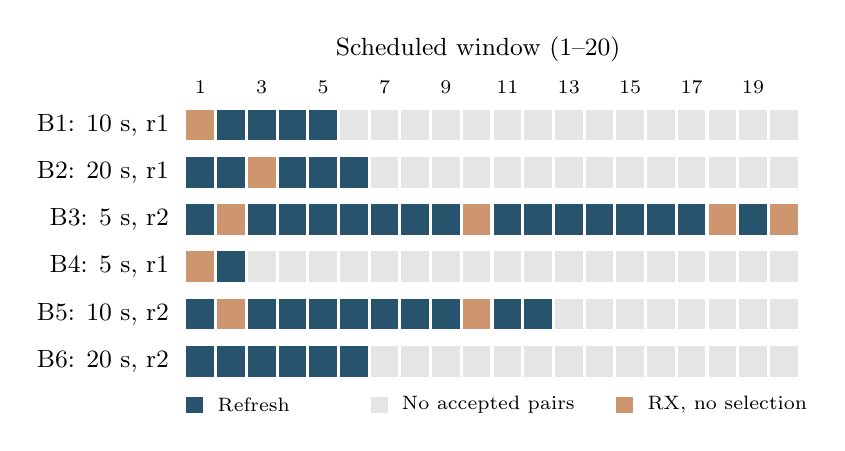
\begin{tikzpicture}[x=0.39cm,y=0.60cm]
\node[anchor=east,font=\small] at (-.25,5) {B1: 10 s, r1};
\fill[studyorange!65] (0,4.675) rectangle ++(.90,.65);
\fill[studyblue] (1,4.675) rectangle ++(.90,.65);
\fill[studyblue] (2,4.675) rectangle ++(.90,.65);
\fill[studyblue] (3,4.675) rectangle ++(.90,.65);
\fill[studyblue] (4,4.675) rectangle ++(.90,.65);
\fill[gray!20] (5,4.675) rectangle ++(.90,.65);
\fill[gray!20] (6,4.675) rectangle ++(.90,.65);
\fill[gray!20] (7,4.675) rectangle ++(.90,.65);
\fill[gray!20] (8,4.675) rectangle ++(.90,.65);
\fill[gray!20] (9,4.675) rectangle ++(.90,.65);
\fill[gray!20] (10,4.675) rectangle ++(.90,.65);
\fill[gray!20] (11,4.675) rectangle ++(.90,.65);
\fill[gray!20] (12,4.675) rectangle ++(.90,.65);
\fill[gray!20] (13,4.675) rectangle ++(.90,.65);
\fill[gray!20] (14,4.675) rectangle ++(.90,.65);
\fill[gray!20] (15,4.675) rectangle ++(.90,.65);
\fill[gray!20] (16,4.675) rectangle ++(.90,.65);
\fill[gray!20] (17,4.675) rectangle ++(.90,.65);
\fill[gray!20] (18,4.675) rectangle ++(.90,.65);
\fill[gray!20] (19,4.675) rectangle ++(.90,.65);
\node[anchor=east,font=\small] at (-.25,4) {B2: 20 s, r1};
\fill[studyblue] (0,3.675) rectangle ++(.90,.65);
\fill[studyblue] (1,3.675) rectangle ++(.90,.65);
\fill[studyorange!65] (2,3.675) rectangle ++(.90,.65);
\fill[studyblue] (3,3.675) rectangle ++(.90,.65);
\fill[studyblue] (4,3.675) rectangle ++(.90,.65);
\fill[studyblue] (5,3.675) rectangle ++(.90,.65);
\fill[gray!20] (6,3.675) rectangle ++(.90,.65);
\fill[gray!20] (7,3.675) rectangle ++(.90,.65);
\fill[gray!20] (8,3.675) rectangle ++(.90,.65);
\fill[gray!20] (9,3.675) rectangle ++(.90,.65);
\fill[gray!20] (10,3.675) rectangle ++(.90,.65);
\fill[gray!20] (11,3.675) rectangle ++(.90,.65);
\fill[gray!20] (12,3.675) rectangle ++(.90,.65);
\fill[gray!20] (13,3.675) rectangle ++(.90,.65);
\fill[gray!20] (14,3.675) rectangle ++(.90,.65);
\fill[gray!20] (15,3.675) rectangle ++(.90,.65);
\fill[gray!20] (16,3.675) rectangle ++(.90,.65);
\fill[gray!20] (17,3.675) rectangle ++(.90,.65);
\fill[gray!20] (18,3.675) rectangle ++(.90,.65);
\fill[gray!20] (19,3.675) rectangle ++(.90,.65);
\node[anchor=east,font=\small] at (-.25,3) {B3: 5 s, r2};
\fill[studyblue] (0,2.675) rectangle ++(.90,.65);
\fill[studyorange!65] (1,2.675) rectangle ++(.90,.65);
\fill[studyblue] (2,2.675) rectangle ++(.90,.65);
\fill[studyblue] (3,2.675) rectangle ++(.90,.65);
\fill[studyblue] (4,2.675) rectangle ++(.90,.65);
\fill[studyblue] (5,2.675) rectangle ++(.90,.65);
\fill[studyblue] (6,2.675) rectangle ++(.90,.65);
\fill[studyblue] (7,2.675) rectangle ++(.90,.65);
\fill[studyblue] (8,2.675) rectangle ++(.90,.65);
\fill[studyorange!65] (9,2.675) rectangle ++(.90,.65);
\fill[studyblue] (10,2.675) rectangle ++(.90,.65);
\fill[studyblue] (11,2.675) rectangle ++(.90,.65);
\fill[studyblue] (12,2.675) rectangle ++(.90,.65);
\fill[studyblue] (13,2.675) rectangle ++(.90,.65);
\fill[studyblue] (14,2.675) rectangle ++(.90,.65);
\fill[studyblue] (15,2.675) rectangle ++(.90,.65);
\fill[studyblue] (16,2.675) rectangle ++(.90,.65);
\fill[studyorange!65] (17,2.675) rectangle ++(.90,.65);
\fill[studyblue] (18,2.675) rectangle ++(.90,.65);
\fill[studyorange!65] (19,2.675) rectangle ++(.90,.65);
\node[anchor=east,font=\small] at (-.25,2) {B4: 5 s, r1};
\fill[studyorange!65] (0,1.675) rectangle ++(.90,.65);
\fill[studyblue] (1,1.675) rectangle ++(.90,.65);
\fill[gray!20] (2,1.675) rectangle ++(.90,.65);
\fill[gray!20] (3,1.675) rectangle ++(.90,.65);
\fill[gray!20] (4,1.675) rectangle ++(.90,.65);
\fill[gray!20] (5,1.675) rectangle ++(.90,.65);
\fill[gray!20] (6,1.675) rectangle ++(.90,.65);
\fill[gray!20] (7,1.675) rectangle ++(.90,.65);
\fill[gray!20] (8,1.675) rectangle ++(.90,.65);
\fill[gray!20] (9,1.675) rectangle ++(.90,.65);
\fill[gray!20] (10,1.675) rectangle ++(.90,.65);
\fill[gray!20] (11,1.675) rectangle ++(.90,.65);
\fill[gray!20] (12,1.675) rectangle ++(.90,.65);
\fill[gray!20] (13,1.675) rectangle ++(.90,.65);
\fill[gray!20] (14,1.675) rectangle ++(.90,.65);
\fill[gray!20] (15,1.675) rectangle ++(.90,.65);
\fill[gray!20] (16,1.675) rectangle ++(.90,.65);
\fill[gray!20] (17,1.675) rectangle ++(.90,.65);
\fill[gray!20] (18,1.675) rectangle ++(.90,.65);
\fill[gray!20] (19,1.675) rectangle ++(.90,.65);
\node[anchor=east,font=\small] at (-.25,1) {B5: 10 s, r2};
\fill[studyblue] (0,0.675) rectangle ++(.90,.65);
\fill[studyorange!65] (1,0.675) rectangle ++(.90,.65);
\fill[studyblue] (2,0.675) rectangle ++(.90,.65);
\fill[studyblue] (3,0.675) rectangle ++(.90,.65);
\fill[studyblue] (4,0.675) rectangle ++(.90,.65);
\fill[studyblue] (5,0.675) rectangle ++(.90,.65);
\fill[studyblue] (6,0.675) rectangle ++(.90,.65);
\fill[studyblue] (7,0.675) rectangle ++(.90,.65);
\fill[studyblue] (8,0.675) rectangle ++(.90,.65);
\fill[studyorange!65] (9,0.675) rectangle ++(.90,.65);
\fill[studyblue] (10,0.675) rectangle ++(.90,.65);
\fill[studyblue] (11,0.675) rectangle ++(.90,.65);
\fill[gray!20] (12,0.675) rectangle ++(.90,.65);
\fill[gray!20] (13,0.675) rectangle ++(.90,.65);
\fill[gray!20] (14,0.675) rectangle ++(.90,.65);
\fill[gray!20] (15,0.675) rectangle ++(.90,.65);
\fill[gray!20] (16,0.675) rectangle ++(.90,.65);
\fill[gray!20] (17,0.675) rectangle ++(.90,.65);
\fill[gray!20] (18,0.675) rectangle ++(.90,.65);
\fill[gray!20] (19,0.675) rectangle ++(.90,.65);
\node[anchor=east,font=\small] at (-.25,0) {B6: 20 s, r2};
\fill[studyblue] (0,-0.325) rectangle ++(.90,.65);
\fill[studyblue] (1,-0.325) rectangle ++(.90,.65);
\fill[studyblue] (2,-0.325) rectangle ++(.90,.65);
\fill[studyblue] (3,-0.325) rectangle ++(.90,.65);
\fill[studyblue] (4,-0.325) rectangle ++(.90,.65);
\fill[studyblue] (5,-0.325) rectangle ++(.90,.65);
\fill[gray!20] (6,-0.325) rectangle ++(.90,.65);
\fill[gray!20] (7,-0.325) rectangle ++(.90,.65);
\fill[gray!20] (8,-0.325) rectangle ++(.90,.65);
\fill[gray!20] (9,-0.325) rectangle ++(.90,.65);
\fill[gray!20] (10,-0.325) rectangle ++(.90,.65);
\fill[gray!20] (11,-0.325) rectangle ++(.90,.65);
\fill[gray!20] (12,-0.325) rectangle ++(.90,.65);
\fill[gray!20] (13,-0.325) rectangle ++(.90,.65);
\fill[gray!20] (14,-0.325) rectangle ++(.90,.65);
\fill[gray!20] (15,-0.325) rectangle ++(.90,.65);
\fill[gray!20] (16,-0.325) rectangle ++(.90,.65);
\fill[gray!20] (17,-0.325) rectangle ++(.90,.65);
\fill[gray!20] (18,-0.325) rectangle ++(.90,.65);
\fill[gray!20] (19,-0.325) rectangle ++(.90,.65);
\node[font=\scriptsize] at (0.45,5.8) {1};
\node[font=\scriptsize] at (2.45,5.8) {3};
\node[font=\scriptsize] at (4.45,5.8) {5};
\node[font=\scriptsize] at (6.45,5.8) {7};
\node[font=\scriptsize] at (8.45,5.8) {9};
\node[font=\scriptsize] at (10.45,5.8) {11};
\node[font=\scriptsize] at (12.45,5.8) {13};
\node[font=\scriptsize] at (14.45,5.8) {15};
\node[font=\scriptsize] at (16.45,5.8) {17};
\node[font=\scriptsize] at (18.45,5.8) {19};
\node[font=\small] at (9.5,6.6) {Scheduled window (1--20)};
\fill[studyblue] (0,-1.1) rectangle ++(.55,.35);\node[anchor=west,font=\scriptsize] at (0.7,-.925) {Refresh};
\fill[gray!20] (6,-1.1) rectangle ++(.55,.35);\node[anchor=west,font=\scriptsize] at (6.7,-.925) {No accepted pairs};
\fill[studyorange!65] (14,-1.1) rectangle ++(.55,.35);\node[anchor=west,font=\scriptsize] at (14.7,-.925) {RX, no selection};
\end{tikzpicture}
\end{document}
